\documentclass[12pt,notitlepage]{article}

\usepackage[utf8]{inputenc}
\usepackage[english]{babel}

% https://tex.stackexchange.com/questions/11778/modifying-everydisplay-causes-the-align-environment-to-stop-working
\let\displaystyle\textstyle


%
\usepackage[
backend=biber,
giveninits=true,
url=false,
isbn=false,
backref=true,
style=alphabetic,
sorting=ynt,
block=none,
maxcitenames=3,
maxbibnames=100,
]{biblatex}
%
% https://tex.stackexchange.com/questions/20335/proper-casing-in-citation-bibliography-titles-using-biblatex-biber
%\DeclareFieldFormat{titlecase}{\MakeSentenceCase*{#1}}
%
\addbibresource{refs.bib}


\usepackage{amsmath, amsfonts, amssymb, mathtools}
\usepackage[svgnames]{xcolor}
\usepackage{datetime2}
\usepackage[
	colorlinks=true, 
	citecolor={DarkRed}, urlcolor={DarkBlue}, linkcolor={DarkBlue},
]{hyperref}


% https://tex.stackexchange.com/questions/3802/how-to-get-doi-links-in-bibliography
% \usepackage{doi}

% 
\usepackage[version=4]{mhchem}
\mhchemoptions{font=sf}

% http://mirrors.ibiblio.org/CTAN/macros/latex/contrib/siunitx/siunitx.pdf
\usepackage{siunitx}


\usepackage{fullpage}

% Paragraph spacing
\usepackage{parskip}
%\usepackage{enumitem}

% https://ostraya.livejournal.com/250833.html
\usepackage{xspace}

\usepackage{graphicx}
\graphicspath{{../code/data/}{../code/model/}{../code/work/}{../images/}}
\DeclareGraphicsExtensions{.pdf,.eps,.png}

% https://tex.stackexchange.com/questions/202046/width-of-the-caption-of-a-figure
% https://tex.stackexchange.com/questions/29039/how-to-limit-the-figure-caption-width
% https://tex.stackexchange.com/questions/822/change-the-font-of-figure-captions
\usepackage[margin=10px,font={small}]{caption}
% https://tex.stackexchange.com/questions/25879/multiple-captions-for-a-single-figure
\usepackage{subcaption}


% http://www.texfaq.org/FAQ-ftnsect
\usepackage[stable]{footmisc}

% https://tex.stackexchange.com/questions/20792/how-to-superimpose-latex-on-a-picture
\usepackage[percent]{overpic}

%\usepackage{epstopdf}

% Tables (the order matters here)
\usepackage{makecell}
\usepackage{booktabs}
\usepackage{arydshln}

% https://tex.stackexchange.com/questions/109467/footnote-in-tabular-environment
\usepackage{footnote}
\makesavenoteenv{tabular}
\makesavenoteenv{table}

% https://tex.stackexchange.com/questions/10130/use-the-values-of-title-author-and-date-on-a-custom-title-page
\usepackage{authoraftertitle}

% https://en.wikibooks.org/wiki/LaTeX/Footnotes_and_Margin_Notes#Margin_Notes
\usepackage{marginnote}

% For editing purposes:
%\usepackage[margin=10pt]{geometry}

% https://latex.org/forum/viewtopic.php?t=10456
\usepackage{titlesec}
\titleformat{\subsubsection}[runin]% runin puts it in the same paragraph
{\normalfont\bfseries}% formatting commands to apply to the whole heading
{\thesubsubsection}% the label and number
{}% space between label/number and subsection title
{}% formatting commands applied just to subsection title
[.]% punctuation or other commands following subsection title



% https://bitbucket.org/goodnightmath/covariance/src/master/tex/main.tex

%%%%%%%%%%%%%%%%%%%%%%%%%%%%%%%%%%%%%%%%%%%%%%%%%%%%%%%%%%%%%%%%%%%%%%%%%%%%%%%
\providecommand{\TODO}[1]{\textrm{\color{red}TODO: #1}}

% http://tex.stackexchange.com/a/106577/44073
\usepackage{ifthen}
\newcounter{todoindex}\setcounter{todoindex}{0}
\newcommand\ADDTODO[1]{%
	\addtocounter{todoindex}{1}%
	\expandafter\gdef\csname todo\roman{todoindex}\endcsname{#1}%
	%\expandafter\csname todolabel\roman{todoindex}\endcsname
	\label{todolabel\roman{todoindex}}%
}
\renewcommand\TODO[1]{%
	{%
		\ADDTODO{#1}%
		{\textrm{\color{red}TODO(\arabic{todoindex}): #1}}%
	}%
}
\newcommand\CHECK[1]{%
	\ADDTODO{CHECK CLAIM: {#1}}%
	{\color{toverify}#1}%
	\smash{\marginnote{\text{\color{red}*}}}%
}
\newcounter{indextodo}
\newcommand{\SHOWTODOS}{%
	\setcounter{indextodo}{0}%
	\begin{enumerate}
	\item[{\color{red} TODOs:}]
	\whiledo{\value{indextodo} < \value{todoindex}}{%
		\addtocounter{indextodo}{1}%
		\item[\color{red}\arabic{indextodo}.]
		p.\pageref{todolabel\roman{indextodo}}.
		%
		\csname todo\roman{indextodo}\endcsname
	}%
	\end{enumerate}
}
%%%%%%%%%%%%%%%%%%%%%%%%%%%%%%%%%%%%%%%%%%%%%%%%%%%%%%%%%%%%%%%%%%%%%%%%%%%%%%%


%%%%%%%%%%%%%%%%%%%%%%%%%%%%%%%%%%%%%%%%%%%%%%%%%%%%%%%%%%%%%%%%%%%%%%%%%%%%%%%
\providecommand{\CODE}[1]{\href{#1}{code}}
\providecommand{\SHOWCODES}{}

% !
\usepackage[strings]{underscore}

\newcommand\codeprefix{https://github.com/numpde/optimum/blob/main/}

% http://tex.stackexchange.com/a/106577/44073
\usepackage{ifthen}
\newcounter{codeindex}\setcounter{codeindex}{0}
\newcommand\ADDCODE[1]{%
	\addtocounter{codeindex}{1}%
	\expandafter\gdef\csname code\roman{codeindex}\endcsname{#1}%
	\label{codelabel\roman{codeindex}}%
}
%
\newcommand{\codereref}[1]{%
\href{\codeprefix\csname code\expandafter\romannumeral#1\endcsname}{%
\color{gray}\##1}}
%
\renewcommand\CODE[1]{%
	{%
		%\ADDCODE{\href{\codeprefix#1}{\texttt{#1}}}%
		\ADDCODE{#1}%
		{\href{\codeprefix#1}{\color{gray}\#\arabic{codeindex}}}%
	}%
}
%
\newcount\fooo
\newcounter{indexcode}
\long\def\addto#1#2{\expandafter\def\expandafter#1\expandafter{#1#2}}
\renewcommand{\SHOWCODES}{%
	\def\tabledata{}
	\setcounter{indexcode}{0}%
	\fooo=0\loop\advance\fooo+1
		\addto\tabledata{%
			\addtocounter{indexcode}{1}%
			\#\arabic{indexcode} &
			p.\pageref{codelabel\roman{indexcode}} &
			\href{\codeprefix\csname code\roman{indexcode}\endcsname}{\texttt{\csname code\roman{indexcode}\endcsname}} \\ 
		}
	\ifnum \fooo < \thecodeindex
	\repeat
	
	\begin{tabular}{c|c|c}
		 & page & \url{\codeprefix} ... \\
		\hline
		\tabledata
	\end{tabular}
}
%%%%%%%%%%%%%%%%%%%%%%%%%%%%%%%%%%%%%%%%%%%%%%%%%%%%%%%%%%%%%%%%%%%%%%%%%%%%%%%




\renewcommand{\d}{\mathrm{d}}
\newcommand{\ddt}{\frac{\d}{\d{t}}}

\newcommand{\TEXT}[1]{\quad\text{#1}\quad}
\newcommand{\with}{\text{$\,{:}\,$}}

\newcommand{\cbra}[1]{{\ensuremath{\color{gray}{#1}}}}
\newcommand{\signal}[1]{{{\cbra{\langle}\ce{#1}\cbra{\rangle}}}}
\newcommand{\protein}[1]{{{\cbra{(}\ce{#1}\cbra{)}}}}
\newcommand{\promoter}[1]{{{\cbra{[}\ce{#1}\cbra{]}}}}

% https://tex.stackexchange.com/questions/543953/arrow-with-blunted-end-head-in-math-mode
\newcommand{\act}{\ {\ensuremath{\mathbin{\to}}}\ }
\newcommand{\rep}{\ {\ensuremath{\mathrel{\raisebox{-.3ex}{\rotatebox{90}{\scalebox{1}[1.2]{$\bot$}}}}}}\ }

\def\[#1\]{\begin{align}#1\end{align}}

% https://tex.stackexchange.com/questions/114113/how-to-label-text-with-equation-number
\newcommand{\eqnum}{\leavevmode\hfill\refstepcounter{equation}\textup{{(\theequation)}}}

\newcommand{\starlink}[1]{\textsuperscript{\makebox[0pt]{\href{#1}{\color{white}$\star$}}}}

\newcommand{\hh}[1]{{\color{Purple}#1}}
\newcommand{\ra}[1]{{\color{Blue}#1}\marginnote{\TODO{review}}}


\title{%
	[DRAFT]\\%
	On-demand public transport is making us mobile
}
\author{RA}
\date{\today}
\newcommand{\linktodoc}{http://bit.ly/}


\makeatletter
\newcommand\footnoteref[1]{\protected@xdef\@thefnmark{\ref{#1}}\@footnotemark}
\makeatother


\begin{document}

\maketitle

\section{Introduction}

The TLC trip record data%
\footnote{\href{https://www1.nyc.gov/site/tlc/about/tlc-trip-record-data.page}{\texttt{https://www1.nyc.gov/site/tlc/about/tlc-trip-record-data.page}}}
records 
Yellow and Green taxi
and other ``for-hire vehicle''
trips 
in New York City.
%
In the earlier years
in particular,
Yellow and Green taxi records
contain timestamps,
trip distance, 
passenger count,
fare, etc.,
but also
approximate locations of pickup and dropoff.
%
%
Based on those data
we give a partial answer to the question
\begin{quote}
	How many small buses could serve the same demand?
\end{quote}

%



Conventions.
%
%
The number in the margin refers to the corresponding code listed in \S\ref{s:code}.


%Abbreviations.
%

\section{Data preparation}

\subsection{Taxi trips\footnote{\label{f:oldcode}The codes for this section were mostly written in 2019.}}

\label{s:trips}

We focus henceforth on May 2016
where 
$\sim$12M (Yellow) and $\sim$1.5M (Green)
trip records are available.
%
The $\sim$11M ``for-hire vehicle'' records
bear no useful details for our purpose.
%
%
%
We keep only 
the trips that begin and end in \href{https://www.openstreetmap.org/search?query=manhattan}{Manhattan}
with
reported trip distance between 0.1 and 30 miles.
%
We filter out records that
lack geo-coordinates.
%
\marginnote{\CODE{code/data/20210610-NYCTLC/a_download.py}}
%
See Fig.~\ref{f:nyctlc} for a net summary.
%
%


\begin{figure}[!p]
    \begin{subfigure}{\linewidth}
		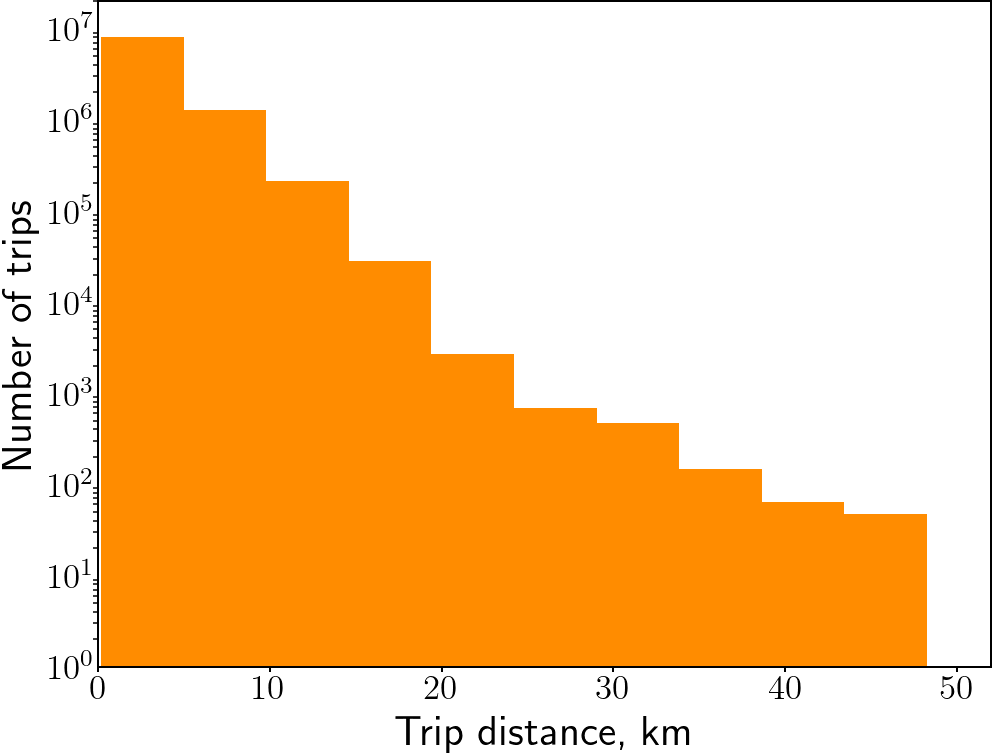
\includegraphics[width=0.49\textwidth]{20210610-NYCTLC/e_explore/trip_distance_histogram/yellow_tripdata_2016-05}
		\hfill
		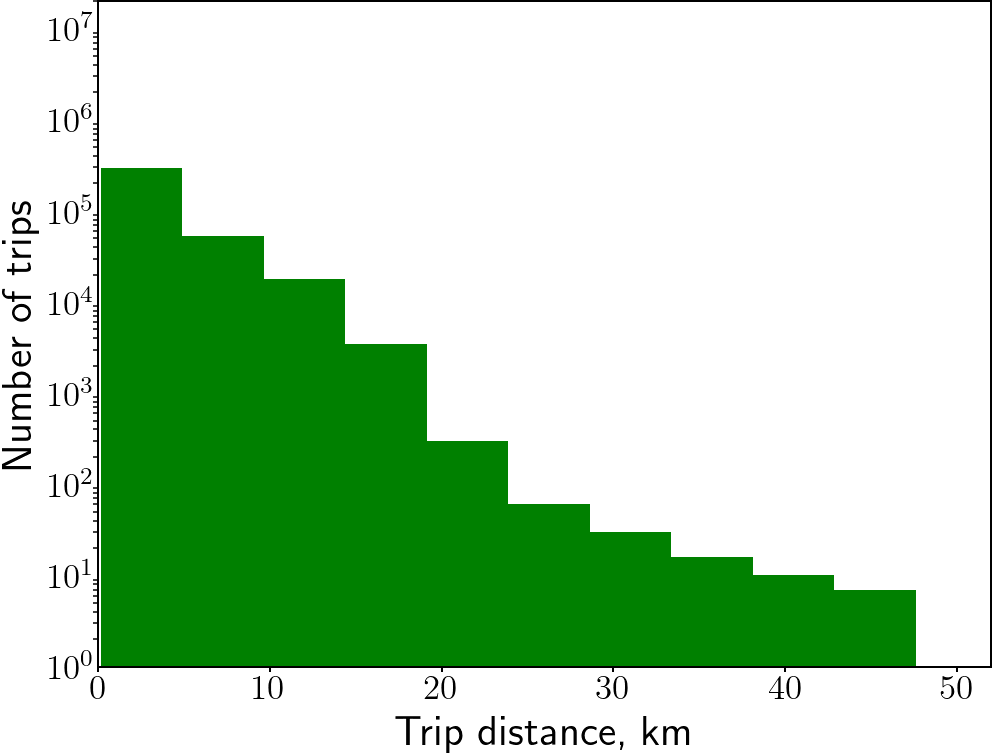
\includegraphics[width=0.49\textwidth]{20210610-NYCTLC/e_explore/trip_distance_histogram/green_tripdata_2016-05}
	
		\caption{Reported trip distance histogram.}
		\label{f:nyctlc-disthist}
	\end{subfigure}
	
	\vspace{\baselineskip}
	
    \begin{subfigure}{\linewidth}
		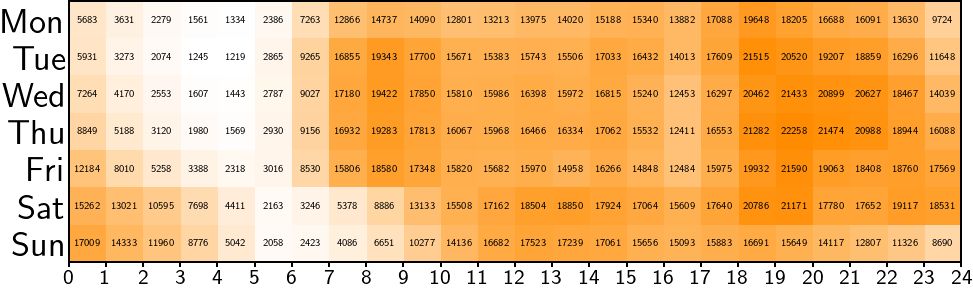
\includegraphics[width=0.49\textwidth]{20210610-NYCTLC/e_explore/pickup_hour_heatmap/yellow_tripdata_2016-05}
		\hfill
		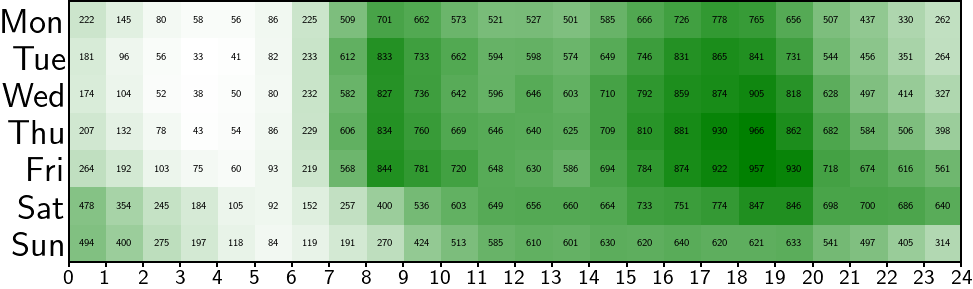
\includegraphics[width=0.49\textwidth]{20210610-NYCTLC/e_explore/pickup_hour_heatmap/green_tripdata_2016-05}
		
		\caption{Pickup hour heatmap.}
		\label{f:nyctlc-pickup}
	\end{subfigure}
	
		
	\vspace{0.25\baselineskip}%
	\marginnote{{\protect\CODE{code/data/20210610-NYCTLC/e_explore.py}}}%
	\vspace{-0.25\baselineskip}
	
	\caption{%
		%\protect\TODO{CAPTION}
		%
		Summary 
		of 
		Yellow ($\nwarrow$) and Green ($\nearrow$) taxi trips 
		filtered as in \S\ref{s:trips}.
	}
	%
	\label{f:nyctlc}
\end{figure}



\subsection{Road graph${}^{\ref{f:oldcode}}$} 
\label{s:graph}



We obtained the road network for Manhattan
\marginnote{\CODE{code/data/20210611-OSM/a_osm_download.py}}%
from the OpenStreetMap Overpass API%
\footnote{\href{https://wiki.openstreetmap.org/wiki/Overpass_API}{\texttt{https://wiki.openstreetmap.org/wiki/Overpass_API}}}
%
and filtered for roads that can plausibly sustain public traffic.
%
\marginnote{\CODE{code/data/20210611-OSM/c_road_graph.py}}
%
It is represented as a digraph,
i.e.~%
there are one-way roads 
and
the routing $A \to B$ differs from $B \to A$.
%
%
When modeling individual trips,
their reported pickup and dropoff locations
are snapped to the nearest node of the road graph;
we ignore about 10\% of the trips 
where the discrepancy is over \SI{20}{m}.

%

The map graphics are from MapBox.
\marginnote{\CODE{code/helpers/opt_maps/maps.py}}



\subsection{Traffic model} \label{s:traffic}

The trip trajectories are not available,
only the pickup and dropoff locations
(with potential GPS uncertainty of 10 to \SI{100}{m}).
%
%
We leverage the reported trip duration to
infer plausible mean-field travel velocities 
(see Fig.~\ref{f:mfv})
throughout the road graph
iteratively as follows.
%
The velocities on all roads are initialized to \SI{5}{m/s}.
%
For a sample of trips that start at 18-19h
the quickest trajectories are estimated.
%
The velocities of the road bits participating in those trajectories
are adjusted toward the reported trip duration.
%
This is repeated.
%
%
\marginnote{\CODE{code/model/20210613-GraphWithLag/b_train.py}}
%
%

The adaptive routes we calculate below
are the quickest trajectories
w.r.t.~this traffic model.


\begin{figure}[!p]
	\begin{subfigure}{0.32\linewidth}
		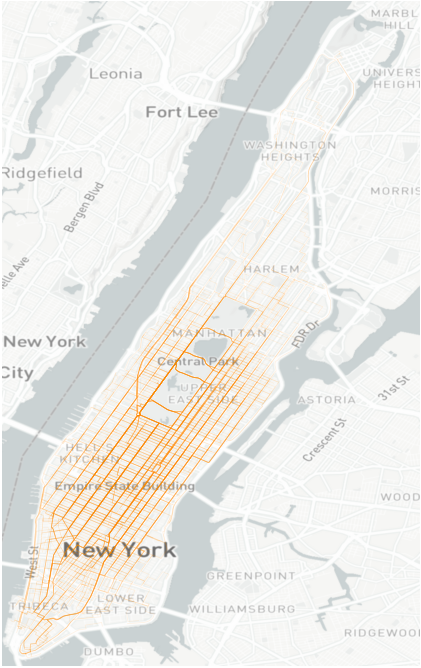
\includegraphics[width=\textwidth]{20210611-OSM/e_explore/trip_trajectories_ingraph/yellow_tripdata_2016-05.png}
		
		\caption{Sample Yellow taxi trips.}
	\end{subfigure}
	\hfill
	\begin{subfigure}{0.32\linewidth}
		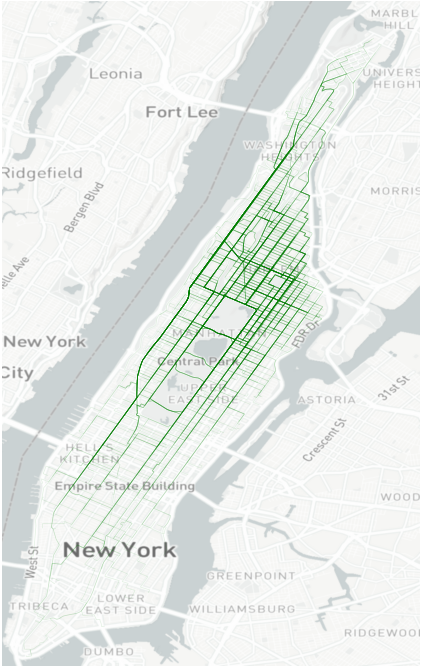
\includegraphics[width=\textwidth]{20210611-OSM/e_explore/trip_trajectories_ingraph/green_tripdata_2016-05.png}
		
		\caption{Sample Green taxi trips.}
	\end{subfigure}
	\hfill
	\begin{subfigure}{0.32\linewidth}
		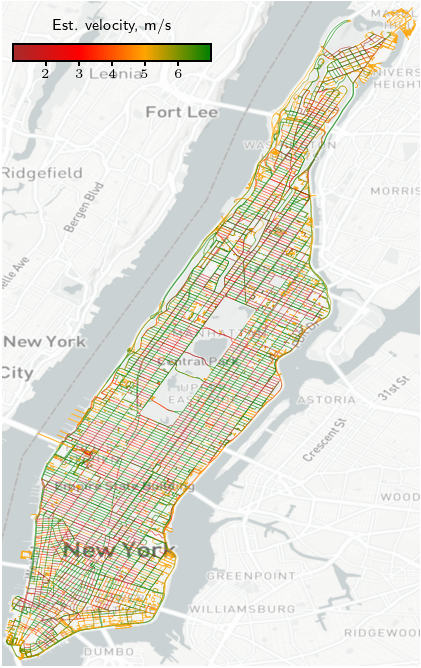
\includegraphics[width=\textwidth]{20210613-GraphWithLag/b_train/v1/lag/H=18/UTC-20210615-132827/train/velocity_i=9.png}
		
		\caption{Inferred mean-field velocity.}
		\label{f:mfv}
	\end{subfigure}
		
	\vspace{0.25\baselineskip}%
	\marginnote{%
		{\protect\CODE{code/data/20210611-OSM/e_explore.py}}, {\protect\CODE{code/model/20210613-GraphWithLag/b_train.py}}
	}%
	\vspace{-0.25\baselineskip}

	\caption{%
		A sample of shortest-path trajectories (\S\ref{s:trips}/\S\ref{s:graph})
		and
		the traffic model from \S\ref{s:traffic}.
	}
			
\end{figure}



\section{Optimization problem}

We are facing
a so-called vehicle routing problem with these main attributes:
%
\begin{itemize}
\item
	Capacitated.
	%
	There are $N$ buses of maximal capacity of $C$ passengers each.
\item
	Time windows.
	%
	Each passenger has to be picked up
	within $[-\SI{2}{min}, \SI{5}{min}]$
	of
	the recorded pickup time in the trip data (\S\ref{s:trips}).
	%
	The dropoff time window extends to $\SI{10}{min}$
	after the recorded dropoff.
	%
	To ensure feasibility,
	a passenger may be ignored 
	at a certain penalty to the optimization objective.	
	%
	The buses are allowed to wait up to $\SI{10}{min}$
	at any location.
\item
	Depot.
	%
	All buses start and finish at a certain location
	but have enough time to reach anywhere
	without compromising feasibility.
%	(hence this is not very important).
\end{itemize}

%

This is difficult in general.
%
We use \texttt{ortools}%
\footnote{\href{https://developers.google.com/optimization/routing/vrp}{https://developers.google.com/optimization/routing/vrp}}
to find reasonable solutions computationally.
%
We can roughly assess optimality
by allotting more time to the solver.
%
%
We compare ``customer satisfaction''
across different fleet sizes $N$ and bus capacities $C$.

%

To obtain reasonable solutions
on modest hardware
we focus on a small slice of 
the trip data at a time,
i.e.~%
a few hundred passengers $\times$ one hour $\times$ a few square kilometers.

%

We pretend here that the demand
and the traffic conditions
are known in advance,
whereas some \SI{10}{min} in advance
would be more realistic.
%
Meanwhile, the density of requests in space and time is quite high.
%
Thus, we believe our results remain informative.


\section{Case study} \label{s:case}

\subsection{Times Square}


%
%
We take%
\marginnote{\CODE{code/work/20210616-OPT1}}
all single-passenger trips with pickup and dropoff 
within $R = \SI{1}{km}$
of Times Square
that 
are reported to start and end
within 18:00--19:00 on May 1, 2016.
%




%%% BIBLIOGRAPHY %%%

\clearpage
\renewcommand*{\bibfont}{\normalfont\small}
\printbibliography % biblatex



\clearpage


\section{Appendix}

\subsection{List of codes} \label{s:code}

\begin{center}
\SHOWCODES
\end{center}


\clearpage\SHOWTODOS



\leavevmode\vfill{\tiny\color{lightgray}\hfill{\DTMnow}}
\end{document}
